% copyright arturo salinas-aguayo 2024
\documentclass[12pt]{article}

\usepackage{graphicx}
\usepackage{amsmath}
\usepackage{amssymb}
\usepackage{array}
\usepackage{amsfonts}
\usepackage{fancyhdr}
\usepackage{geometry}
\usepackage{subfigure}
\usepackage{caption}
\usepackage{tikz}
\usepackage{bm}
\usepackage{float}

\geometry{letterpaper, margin=1in}
\graphicspath{ {../images/} }

% Header and Footer
\pagestyle{fancy}
\fancyhf{}
\fancyhead[L]{CSE 2500-01: Homework 4}
\fancyhead[R]{Page \thepage}
\setlength{\headheight}{15pt}

\author{Arturo Salinas-Aguayo}
\title{CSE 2500-01: Homework 4}
% theorem set
\newtheorem{example}{Example}
% Example block environment
\newenvironment{examp}
{\vspace{0.5cm}
 \hrule
\vspace{0.5cm}
\begin{example}}
{\hrule
\vspace{0.5cm}
\end{example}}

\begin{document}
\newcommand{\closure}[2][3]{%
	{}\mkern#1mu\overline{\mkern-#1mu#2}}
\newcommand\ncoverline[1]{\mkern1mu\overline{\mkern-1mu#1\mkern-1mu}\mkern1mu}
% Title Page
\begin{titlepage}
	\centering
	\vspace*{3cm}
	\huge\textbf{CSE 2500-01: Homework 4}\\
	\vspace{5cm}
	\Large\textbf{Arturo Salinas-Aguayo}\\
	\normalsize
	Spring 2025\\
	Electrical and Computer Engineering Department\\
	\vfill
	
\includegraphics[scale=0.1]{uconnlogo}\\
	College of Engineering, University of Connecticut\\
	\scriptsize{Coded in \LaTeX}
	\vspace*{1cm}
\end{titlepage}

\section*{Problems}
\subsection*{Question 1.}
Let $B(x)$ be ``$-10 < x < 10$." Find the truth set of $B(x)$ for each of the following domains:
\begin{enumerate}
	\item[(a)] $\mathbb{Z}$
	      \[
		      \{-9, -8, -7, -6, -5, -4, -3, -2, -1, 0, 1, 2, 3, 4, 5, 6, 7, 8, 9\}
	      \]
	\item[(b)] $\mathbb{Z}^{+}$
	      \[
		      \{1, 2, 3, 4, 5, 6, 7, 8, 9\}
	      \]
	\item[(c)] The set of all even integers
	      \[
		      \{ -8, -6, -4, -2, 0, 2, 4, 6, 8\}
	      \]

\end{enumerate}

\subsection*{Question 2.}
Rewrite each of the following statements in the form "$\forall x, \text{if} \_\_\_ \text{then} \_\_\_$".
\begin{enumerate}
	\item[(a)] All Python programs have at least 5 lines.

	      \(\forall\) \(x\), if \(x\) is a Python program, then \(x\) has at least 5 lines.
	\item[(b)] Any valid argument with true premises has a true conclusion.

	      \(\forall\) \(x\), if \(x\) is a valid argument with true premises, then \(x\) has a true conclusion.
\end{enumerate}

\subsection*{Question 3.}
Rewrite the following statement in two forms:
\begin{enumerate}
	\item[(a)] "$\exists x$ such that \_\_\_"
	\item[(b)] "$\exists x$ such that \_\_\_ and \_\_\_"
\end{enumerate}
where the statement is "Some questions are easy."

\begin{enumerate}
	\item[(a)]
	      \(\exists\) a question \(x\) such that \(x\) is easy.
	\item[(b)]
	      \(\exists\) \(x\) such that \(x\) is a question and \(x\) is easy.
\end{enumerate}

\subsection*{Question 4.}
Write a negation for each statement:
\begin{enumerate}
	\item[(a)] $\forall$ real number $x$, if $x^2 \geq 1$ then $x > 0$.

	      \(\exists\) a real number \(x\) such that \(x^2 \geq 1\) and \(x \ngtr 0\).
	\item[(b)] $\forall n \in \mathbb{Z}$, if $n$ is prime then $n$ is odd or $n = 2$.

	      \(\exists\) n \(\in  \mathbb{Z}\), such that if \(n\) is prime and is not odd and \(n\) \(\ne 2\).
\end{enumerate}

\subsection*{Question 5.}
Rewrite each statement in if-then form:
\begin{enumerate}
	\item[(a)] Being divisible by 8 is a sufficient condition for being divisible by 4.

	      If an integer is divisible by 8, then it is divisible by 4.

	\item[(b)] Passing a comprehensive exam is a necessary condition for obtaining a master’s degree.

	      If a person obtains a master's degree, then that person has passed a comprehensive exam.
	\item[(c)] A polygon is square only if it has four sides.

	      If a polygon is a square, then it has four sides.
\end{enumerate}

\subsection*{Question 6.}
The following statements refer to Tarski's world (Figure \ref{fig:Tarski}).
\begin{figure}[H]
	\centering
	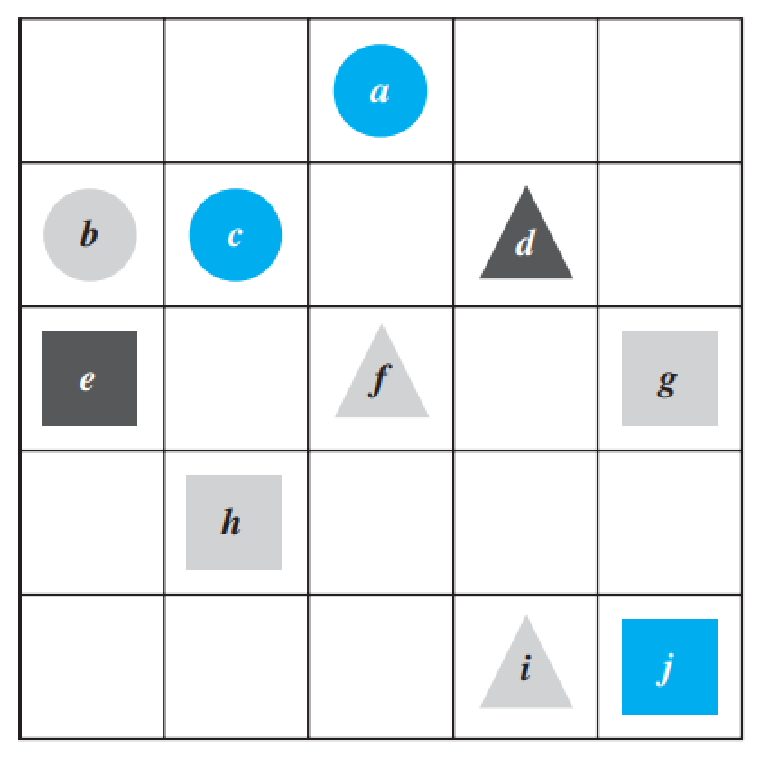
\includegraphics[width=6cm]{tarski}
	\caption{Tarski's World Diagram}
	\label{fig:Tarski}
\end{figure}
For each:
\begin{enumerate}
	\item[(a)] Determine whether the statement is true or false and justify your answer.
	\item[(b)] Write a negation for the statement.
\end{enumerate}
\begin{enumerate}
	\item $\forall$ circle $x$ and $\forall$ square $y$, $x$ is above $y$.

	      \begin{enumerate}
		      \item[(a)] This statement claims that all of the circles happen to be above squares. This is true. The circles are \(b, c\), and \(a\) and the squares are \(e, g\), and \(j\). All of \(b, c, a\) lie above \(e, g, j\).

		      \item[(b)] There is a circle, \(x\) and square \(y\) such that \(x\) is not above \(y\)
	      \end{enumerate}

	\item $\exists$ a circle $x$ and $\exists$ a square $y$ such that $x$ is above $y$ and $x$ and $y$ have the same color.

	      \begin{enumerate}
		      \item[(a)]     This statement claims that there are a circle and square such that the circle is above the square and has teh same color as the square. This is true. For example, the circle \(c\) lies above the square, \(j\) and is the same color: blue.

		      \item[(b)] \(\forall\) circle \(x\) and \(\forall\) square $y$, $x$ is not above $y$ or $x$ and $y$ do not have the same color.
	      \end{enumerate}
\end{enumerate}
\end{document}
